% Faithful vector redraw of nearest-points3.png (627 x 353 pixels).
% Coordinates use the original image's top-left origin; one unit is one pixel.
% Regenerate from this directory:
% latex -interaction=nonstopmode -halt-on-error nearest-points-3.tex
% dvisvgm --no-fonts --exact --bbox=papersize --output=nearest-points-3.svg nearest-points-3.dvi
\documentclass[tikz,border=0pt]{standalone}
\usepackage[T1]{fontenc}
\usepackage{newtxtext,newtxmath}
\begin{document}
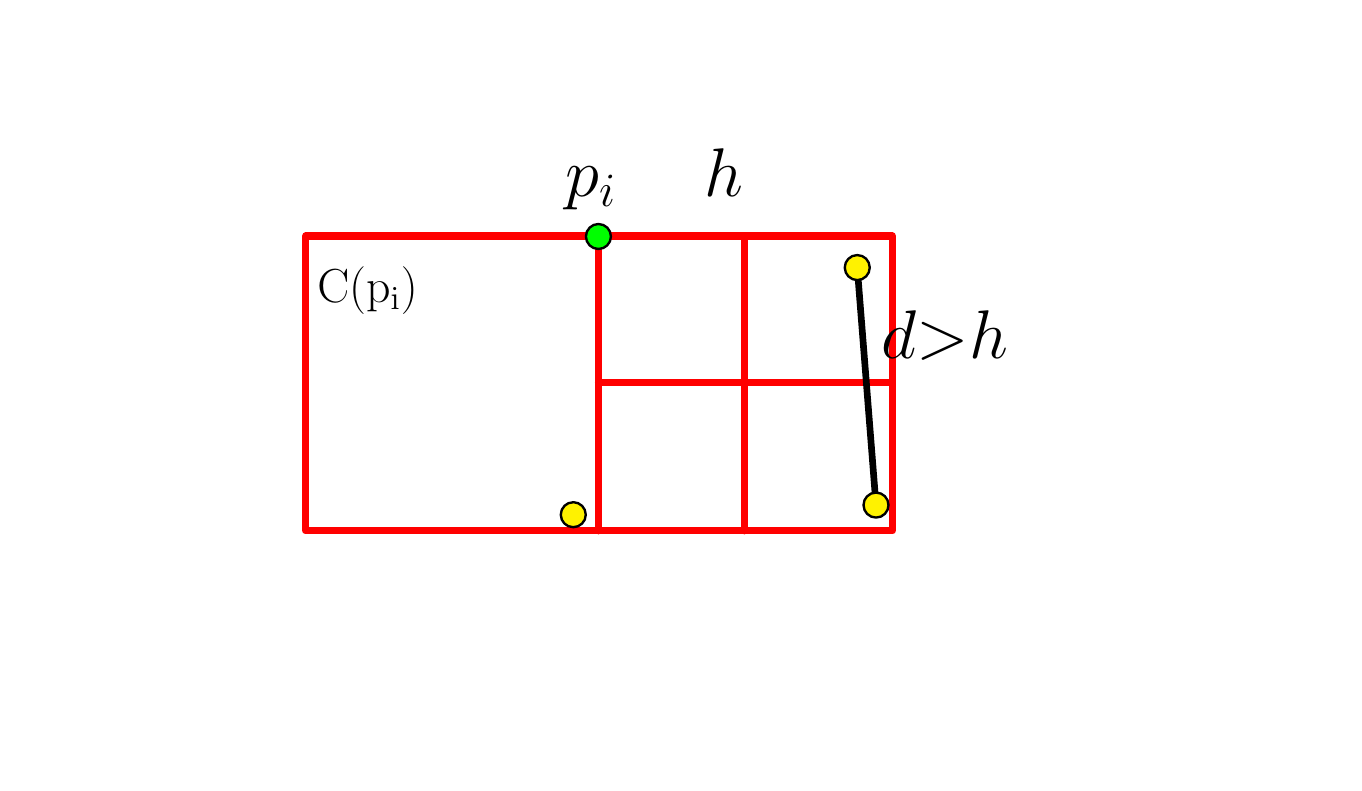
\begin{tikzpicture}[x=0.75bp,y=-0.75bp,
  every node/.style={inner sep=0pt,outer sep=0pt,anchor=base west},
  line cap=round,line join=round]
  \path[use as bounding box] (0,0) rectangle (627,353);
  \clip (0,0) rectangle (627,353);
  \fill[white] (0,0) rectangle (627,353);
  % Preserve the complete rectangle, all four points, and the baseline labels.
  \draw[red,line width=2.6bp] (133.5,100) rectangle (415,241.5)
    (274,100) -- (274,241.5)
    (344,100) -- (344,241.5)
    (274,170.5) -- (415,170.5);
  \draw[black,line width=2.4bp] (398.20,115.15) -- (407.20,229.15);
  \node[font=\fontsize{18bp}{21bp}\selectfont] at (139,132) {$\mathrm{C(p_i)}$};
  \node[font=\fontsize{25bp}{29bp}\selectfont] at (258,81) {$\boldsymbol{p_i}$};
  \node[font=\fontsize{25bp}{29bp}\selectfont] at (325,81) {$\boldsymbol{h}$};
  \node[font=\fontsize{25bp}{29bp}\selectfont] at (410,159) {$\boldsymbol{d}{>}\boldsymbol{h}$};
  \foreach \x/\y in {273.96/100.23} {
    \filldraw[fill=green,draw=black,line width=0.85bp]
      (\x,\y) circle[radius=4.5bp];
  }
  \foreach \x/\y in {398.20/115.15,407.20/229.15,261.89/233.77} {
    \filldraw[fill=yellow,draw=black,line width=0.85bp]
      (\x,\y) circle[radius=4.5bp];
  }
\end{tikzpicture}
\end{document}
